En este capítulo se verá como, dado un conjunto de definiciones de funciones, por medio de razonamiento ecuacional podemos llegar a otras definiciones y/o probarlas. Las pruebas aquí se harán mediantte inducción.

Muchas veces es algo engorroso probar funciones similares repetidamente, por eso veremos una forma de hacer pruebas (en algunos casos) más cortas,
presentando unas \textit{funciones de orden superior} que encapsulan patrones comunes de cómputo. Y así, probar resultados más generales y apelar a ellos.

Al final se verá que la eficiencia también importa, porque se mostrarán algunos ejemplos; como un problema famoso llamado \textit{``The maximum segment sum''}
y una mejora de la función \texttt{scanr}. Y todo esto se logrará como consecuencia de lo dicho anteriormente.

\subsection{Inducción sobre listas}
Recordemos que toda lista finita es de la forma; una lista vacía \texttt{[]} ó \texttt{x:xs} donde \texttt{xs} es una lista finita. Por consiguiente, para probar que $P(xs)$ se mantiene para todas las lista finitas $xs$,
se tiene que probar que:

\begin{enumerate}
    \item $P([])$ se cumple
    \item Para toda $x$ y para todas las listas finitas $xs$, que $P(x:xs)$ se cumple dado que $P(xs)$ también.
\end{enumerate}

Tomemos la definición de concatenación \texttt{(++)},
\inputminted{haskell}{definiciones/concatenation.hs}

Y ahora probemos que (++) es asociativa para todas las listas finitas $xs$, es decir:

(xs ++ ys) ++ zs = xs ++ (ys ++ zs)

Por inducción sobre $xs$:
% TODO: poner aquí lo del strictness property https://stackoverflow.com/questions/27672585/efficient-version-of-inits/27674051#27674051

%{\displaystyle x+5} is the left-hand side (LHS) and {\displaystyle y+8}{\displaystyle y+8} is the right-hand side (RHS).
%FIXME: si caben dos eucaciones por lado lo hago en columnas.

\begin{itemize}
\item Caso []
\begin{minted}{haskell}
(LHS)

([] ++ ys) ++ zs
=   {++.1}
ys ++ zs
\end{minted}

\begin{minted}{haskell}
(RHS)

[] ++ (ys ++ zs)
=   {++.1}
ys ++ zs
\end{minted}

\item Caso (x:xs)
\begin{minted}{haskell}
(LHS)

((x:xs) ++ ys) ++ zs
=   {++.2}
(x:(xs ++ ys)) ++ zs
=   {++.2}
x:((xs ++ ys) ++ zs)
\end{minted}

\begin{minted}{haskell}
(RHS)

(x:xs) ++ (ys ++ zs)
=   {++.2}
x:(xs ++ (ys ++ zs))
=   {induction}
x:((xs ++ ys) ++ zs)
\end{minted}

\end{itemize}

\section{Pliegues}

\subsection{\texttt{foldr}}
\inputminted{haskell}{definiciones/foldr.hs}

\subsection{Síntesis de programas vía la propiedad universal}


\subsection{\texttt{foldl}}
\inputminted{haskell}{definiciones/foldl.hs}



\section{Programación funcional}
De forma muy general y resumiendo, la programación funcional:
\begin{itemize}
    \item es un método de construcción de un programa que hace énfasis en las funciones y sus aplicaciones
    en vez de cómandos y sus ejecuciones.

    \item usa notación matemática simple que permite que los problemas sean descritos de manera clara
    y consisa.
    \item tiene bases matemáticas que fundamentan el razonamiento ecuacional acerca de las propiedades de
    los programas.
\end{itemize}

\section{Definiciones inductivas y recursivas}
%TODO

\section{Razonamiento ecuacional}
%TODO


\section{Definiciones de listas}
%TODO

\section{Definiciones de funciones}
\inputminted{haskell}{definiciones/map.hs}



\section{Ley de Fusión}

\begin{minted}{haskell}
f . foldr g a = foldr h b
\end{minted}

\begin{itemize}
    \item $f$ es una función estricta.
    \item $f a = b$
    \item $f (g y x) = h (f y) x$ para toda $x$ y $y$.w
\end{itemize}

Ejmeplos:
\begin{itemize}
    \item \hsCode{double . sum    = foldr ((+) . double) 0}
    \item \hsCode{length . concat = foldr ((+) . length) 0}
\end{itemize}

% TODO poner lo de una función estrictca, está en el thinking functionally with hskell página 29

%% TODO: poner aquí lo de lados de la ecuación
% https://en.wikipedia.org/wiki/Sides_of_an_equation

% Polymorphic algorithms
% https://wiki.haskell.org/Polymorphism#:~:text=A%20value%20is%20polymorphic%20if,polymorphism%20and%20ad%2Dhoc%20polymorphism

% foldr
% https://wiki.haskell.org/Foldr_Foldl_Foldl'
%http://www.cantab.net/users/antoni.diller/haskell/units/unit06.html

\section{\textit{Scan Lemma}}

En esta sección se considerará la función \hsCode{scanl}, \hsCode{scanl} aplica un pliegue
izquierdo (\hsCode{foldl f e}) a cada segmento (todos los prefijos) de una lista como se muestra
a continuación,

\begin{minted}{haskell}
scanl (@) e [x, y, z, ...] = [e, e@x,(e@x)@y,((e@x)@y)@z,...]
\end{minted}

Se propondrá la siguiente especificación de \hsCode{scanl} como:
\begin{minted}{haskell}
scanl :: (b -> a -> b) -> b -> [a] -> [b]
scanl f e = map (foldl f e) . inits

inits :: [a] -> [[a]]
inits []     = [[]]
inits (x:xs) = [] : map (x:) (inits xs)
\end{minted}

Ejemplo:
\begin{minted}{haskell}
>>> scanl (+) 0 [1..10]
[0,1,3,6,10,15,21,28,36,45,55]
\end{minted}

La expresión anterior calcula la suma de cada prefijo de una lista de números del 1 al 10.
\begin{minted}{haskell}
[0, 0+1, (0+1)+2, ((0+1)+2)+3, (((0+1)+2)+3)+4, ...]
\end{minted}

Veamos un ejemplo de \hsCode{scanl}
\begin{minted}{haskell}
>>> inits [1..5]
[[],[1],[1,2],[1,2,3],[1,2,3,4],[1,2,3,4,5]]
\end{minted}

Pero se puede ver que la definición propuesta de \hsCode{scanl} involucra evaluar \hsCode{f} un
total de $\sum_{i=0}^{n} i = \frac{n(n+1)}{2}$ veces sobre una lista de longitud $n$.

Es aquí cuando uno se pregunta si ¿se podría hacer mejor?. La respuesta es sí, cálculando una mejor
definiciónpor medio de razonamiento ecuacional. Cosideremos por casos.

\begin{itemize}
\item Caso \hsCode{[]}
\begin{minted}{haskell}
scanl f e []
  = -- {Definición de scanl}
map (foldl f e) (inits [])
  = -- {Por inits.1}
map (foldl f e) [[]]
  = -- {Por map.1 y map.2}
(foldl f e []) : map (foldl f e) []
  = -- {Por foldl.1 y map.1}
e : []
  = -- {Azucar sintáctica}
[e]
\end{minted}

Teniendo así que \hsCode{scanl f e [] = [e]}.

\item Caso \hsCode{x:xs}
\begin{minted}{haskell}
scanl f e (x:xs)
  = -- {Definición de scanl}
map (foldl f e) (inits (x:xs))
  = -- {Por inits.2}
map (foldl f e) ([] : map (x:) (inits xs))
  = -- {Por map.1 y map.2}
(foldl f e []) : (map (foldl f e . (x:)) (inits xs))
  = -- {Por foldl.1}
e : (map (foldl f e . (x:)) (inits xs))
  = -- {Por la afrimación que se demostrará abajo y que es el caso (x:xs)}
e : map (foldl f (f e x)) (inits xs)
  = -- {Por la primera definición de scanl.1}
e:scanl f (f e x)
\end{minted}

\textbf{Afirmación:} \hsCode{foldl f e . (x:) = foldl f (f e x)}. Se seguirá como una consecuencia
inmediata de \hsCode{foldl}.

\begin{itemize}
\item Caso \hsCode{x:[]}
\begin{minted}{haskell}
foldl f e . (x:) []
  = -- {Composición de funciones}
foldl f e [x]
  = -- {Aplicación y azucar sintáctica}
foldl f (f e x) []
  = -- {Por foldl.1 y Por foldl.2}
e
\end{minted}

\item Caso \hsCode{x:ys}, análogo al anterior.
\end{itemize}
\end{itemize}

Teniendo así una nueva definición de \hsCode{scanl} como,
\begin{minted}{haskell}
scanl f e []     = [e]
scanl f e (x:xs) = e:scanl f (f e x) xs
\end{minted}

donde \hsCode{f} solo se calcula un número lineal de veces, a diferencia de su primera definición
propuesta que requería un número cuadrático de veces.

Aunque si vemos definición\footnote{
\url{https://hackage.haskell.org/package/base-4.14.1.0/docs/src/GHC.List.html\#scanl}
} del preludio es diferente:
\begin{minted}{haskell}
scanl                   :: (b -> a -> b) -> b -> [a] -> [b]
scanl                   = scanlGo
  where
    scanlGo           :: (b -> a -> b) -> b -> [a] -> [b]
    scanlGo f q ls    = q : (case ls of
                               []   -> []
                               x:xs -> scanlGo f (f q x) xs)
\end{minted}

Pero esto de debe a que la versión que se calculó da \hsCode{scanl f e undefined = undefined} y la
versión de preludio \hsCode{scanl f e undefined = e:undefined}. Esto se debe a que como Haskell
es perezoso, no nos debemos de preguntar nada acerca de la lista a procesar, pero lo que es seguro
es que empieza con \texttt{e}.

En general, cualquier problema que involucre la función \hsCode{inits}, este lema es bastante útil
de saber porque si recordamos la primera especificación:
\begin{minted}{haskell}
scanl f e = map (foldl f e) . inits
\end{minted}

La LHS toma $\Theta(n)$ el número de evaluaciones de \hsCode{f} mientras que RHS toma $\Theta(n^2)$.
Y como se demostró ambas expresiones son equivalentes.

\begin{figure}[h]
\caption{Un ejemplo concreto de la versión propuesta inicialmente de \texttt{scanl} y la que se derivó}
\centering
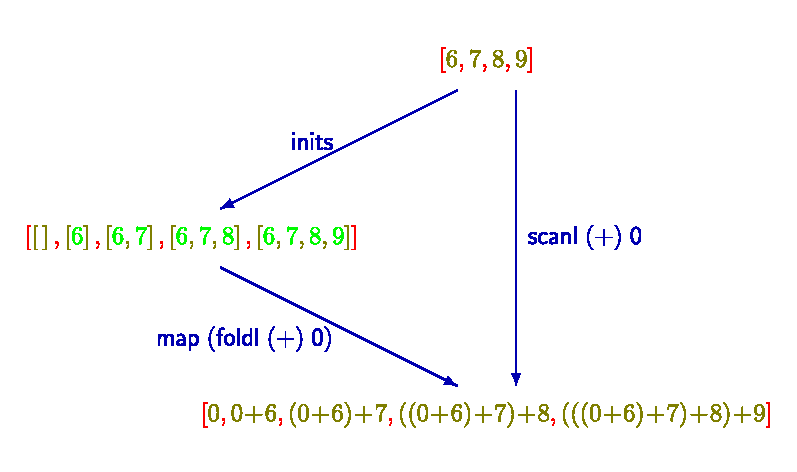
\includegraphics[width=0.9\textwidth]{scan_lemma_example.pdf}
\end{figure}

\subsection{\textit{The maximum segment sum}}
